\section{Linear Transformation}

\section*{\S\ Linear Operator }

\begin{defn}[Linear Transformation]
	Let $V$ and $\mathrm{W}$ be vector spaces (over $\mathrm{F}$). We call a function $\mathrm{T}: \mathrm{V}  \rightarrow  \mathrm{W}$    a linear transformation from $\mathrm{V}$ to $\mathrm{W}$ if, for all x, y $\in$ $\mathrm{V}$ and c $\in$ $\mathrm{F}$, we have

\begin{enumerate}
	\item [$(a)$]   $\mathrm{T}(x + y)$ = $\mathrm{T}(x) + \mathrm{T}(y)$ 
	\item [$(b)$]    $\mathrm{T}$($\mathrm{c}x)$ = $\mathrm{c}\mathrm{T}(x)$
\end{enumerate} 
\end{defn}

\begin{defn}
	Let $\mathrm{T} , \mathrm{U}: \mathrm{V} \rightarrow \mathrm{W}$ be arbitrary functions, where V and W are vector spaces over F, and let $a \in \mathrm{F}$. We define $\mathrm{T}+\mathrm{U} : \mathrm{V} \rightarrow \mathrm{W}$ \ \ by\ \ $(\mathrm{T}+\mathrm{U})(x) = \mathrm{T}(x)+\mathrm{U}(x)$\ \ for all $x \in \mathrm{V}$, and $a\mathrm{T}: \mathrm{V} \rightarrow \mathrm{W}$\ \ by\ \ $(a\mathrm{T})(x) = a\mathrm{T}(x)$\ \ for all \ \ $x \in \mathrm{V}$.
\end{defn}

\begin{rmk*}
	If $F = Q$ then $(a)\Rightarrow(b)$.	
\end{rmk*}

\begin{rmk*}
	If $T : C \rightarrow C$ be function defined by	$T(\delta)=\delta$.  $T$ is additive but not linear.
\end{rmk*}

\begin{prop}
$ $
	\begin{enumerate}
		\item If $T$ is linear, then $T(0)=0$.
		\item $T$ is linear if and only if $T(cx+y) = cT(x) + T(y)$ for all $x, y \in V$ and $c\in F$.
		\item If $T$ is linear, then $T(x-y) = T(x) - T(y)$ for all $x, y \in V$
		\item $T$ is linear if and only if, for $x_1, x_2, \cdots, x_n \in V$ and $a_1, a_2, \cdots, a_n \in F$, we have 
		$$ T(\sum_{i=1}^na_ix_i) = \sum_{i=1}^na_iT(x_i). $$
		\item For all $a\in F, aT + U$ is linear.
		\item Using the operations of addition and scalar multiplication in the preceding definition, the collection of all linear transformations from $V$ to $W$ is a vector space over $F$.
	\end{enumerate}
\end{prop}

\begin{defn}[Null Space, Range]
Let $\mathrm{V}$ and $\mathrm{W}$ be vector spaces and let $\mathrm{T}: \mathrm{V}  \rightarrow  \mathrm{W}$ be linear. We define the null space(or kernel) $N(T)$ of $T$ to be the set of all vectors $x$ in $V$ such that $T(x) = 0$ ; that is , $N(T) = \{x \in V : T(x) = 0\}$. \\  We define the range(or image) $R(T)$ of $T$ to be the subset of $W$consisting of all images (under $T$) of vectors in $V$; that is, $R(T) = \{T(x):x \in V\}$
\end{defn}

\begin{rmk*}
Let $V$ and $W$ be vector spaces, and let $I:V \rightarrow V$ and $ T_0:V \rightarrow W$ be the identity and zero transformations, respectively. Then $N(I) = \{0\}$, $R(I)=V$, $N(T_0)=V$, and $R(T_0)=\{0\}$.	
\end{rmk*}

\begin{thm}
	Let $V$ and $W$ be vector spaces and $\mathrm{T}: \mathrm{V}  \rightarrow  \mathrm{W}$ be linear. Then $N(T)$ and $R(T)$ are subspaces of $\mathrm{V}$ and $\mathrm{W}$, respectively.
\end{thm}

\begin{proof}
	\begin{proof}
	$\\$ Let $0_{V}\in V , 0_{W} \in W$ be a zero vectors \\ $\because T(0_{V}) = 0_{W} \therefore 0_{V}\in N{(T)}$

Let $x,y \in N(T) , c\in F$, \\
$\because T(x+y) = T(x) + T(y) = 0_{W} + 0_{W} = 0_{W}$ \\
$\therefore x + y \in N(T)$ \\
$\because T(cx) = cT(x) = c0_{W} = 0_{W}$\\
$\therefore cx \in N(T)$\\
$\implies N(T)$ is a subspace of $V$\\
$\because T(0_{V}) = 0_{W} \therefore 0_{W} \in R(T)$ \\
Let $x,y \in R(T)$ and $c \in F.$ $\exists   v,w \in V, T(v) = x \in V $ and $T(w) = y$ \\
$\because x + y = T(v) + T(w) = T(v+w)$\\
$\therefore x + y \in R(T)$\\
$\because cx = cT(v) = T(cv)$\\
$\therefore cx \in R(T) \implies R(T)$ is a subspace of $W$	
\end{proof}






\end{proof}


\begin{rmk*}
	Give an example of distinct linear transformations $T$ and $U$ such that $N(T)=N(U)$ and $R(T)=R(U)$
\end{rmk*}

\begin{thm}
Let V and W be vector spaces, and let $\mathrm{T} : \mathrm{V}  \rightarrow \mathrm{W}$ be linear. If $\beta = \{ v_1,v_2,\cdots,v_n \}$ is a basis for $\mathrm{V}$ , then $$ \mathrm{R}(\mathrm{T}) = \mathrm{span}(\mathrm{T}(\beta)) = \mathrm{span}(\{\mathrm{T}(v_1), \mathrm{T}(v_2), . . . , \mathrm{T}(v_n)\})$$	
\end{thm}

\begin{proof}
	\begin{proof}
	$\\$ Clearly, $T(v_{i}) \in R(T)$ \\
$\because R(T)$ is a subspace 
$\therefore$ By thm 1.5 : $span(T(\beta))\subseteq R(T)$ \\
Let $w \in R(T)$\\
$\because w = T(v)$ for some $v \in V$  
$\therefore \beta$ is a basis of $V$ \\
$\therefore v = \sum^{n}_{i=1}a_iv_i$ for some $a_i \in F, \ \ 1\leq i \leq n$\\
$\because T$ is linear 
$\therefore w = T(v) = T(\sum^{n}_{i=1}a_iv_i) = \sum^{n}_{i=1}a_iT(v_i) \in span(T(\beta))$ \\
$\therefore R(T) \subseteq span(T(\beta)) \implies R(T)=span(T(\beta))=span(\{T(v_1),\cdots,T(v_n)\})$
\end{proof}




	%\begin{proof}
	$\\$ Clearly, $T(v_{i}) \in R(T)$ \\
$\because R(T)$ is a subspace 
$\therefore$ By thm 1.5 : $span(T(\beta))\subseteq R(T)$ \\
Let $w \in R(T)$\\
$\because w = T(v)$ for some $v \in V$  
$\therefore \beta$ is a basis of $V$ \\
$\therefore v = \sum^{n}_{i=1}a_iv_i$ for some $a_i \in F, \ \ 1\leq i \leq n$\\
$\because T$ is linear 
$\therefore w = T(v) = T(\sum^{n}_{i=1}a_iv_i) = \sum^{n}_{i=1}a_iT(v_i) \in span(T(\beta))$ \\
$\therefore R(T) \subseteq span(T(\beta)) \implies R(T)=span(T(\beta))=span(\{T(v_1),\cdots,T(v_n)\})$
\end{proof}




\end{proof}


\begin{ex*}
Prove Theorem 2.2 for the case that $\beta$ is infinite, that is, $R(T) = span(\{T(v):v \in \beta\})$. 	
\end{ex*}

\begin{defn}[Nullity and Rank]  
  Let $\mathrm{V}$ and $\mathrm{W}$ be vector spaces and let $ \mathrm{T}: \mathrm{V}  \rightarrow  \mathrm{W}$ be linear. If $N(T)$ and $R(T)$ are finite-dimensional, then we define the nullity of $T$, denoted $nullity(T)$, and the rank of $T$, denoted $rank(T)$, to be the dimensions of $N(T)$ and $R(T)$, respectively.	
\end{defn}

\begin{thm}
	Let V and W be vector spaces,
and let $ \mathrm{T} : \mathrm{V}  \rightarrow  \mathrm{W} $ be linear. \\ If $V$ is finite-dimensional, then
 
 
$$	nullity(T) + rank(T) = dim(V).$$
\end{thm}

\begin{proof}
$\\$ Suppose $\dim(V)=n,$ $\dim(N(T))=k$ and $\{v_i = \forall_i = 1,\cdots,k \}$ is a basis of $N(T)$\\
$\because$ Cor of thm 1.11 $\therefore$ We can extend $\{v_i:$ for $i = 1,\cdots,k\}$ to a basis $\beta = \{v_i:$ for $i = 1,\cdots,k\}$ of $V$\\
Claim : $S = \{T(v_i):$ for $i = k+1, \cdots, n\}$ is a basis of $R(T)$
\begin{enumerate}
	\item Claim $span(S) = R(T)$ \\ 
	$\because$ Thm 2.2 
	$\therefore R(T) = span(T(\beta)) = span(\{T(v_1), \cdots , T(v_n)\})$\\
	$\because T(v_i) = 0$ for $i=1, \cdots, k$\\
	$\therefore R(T) = span(\{T(v_{k+1}, \cdots, T(v_n)\}) = span(S)$ 
	\item Claim : S is linear independent \\
	Suppose $\sum^n_{i=k+1}b_iT(v_i)=0 \ \ \forall b_{k+1}, \cdots b_n \in F$ \\
	$\because$ T is linear $\therefore T (\sum^n_{i=k+1}b_iv_i)=0 \implies \sum^n_{i=k+1}b_iv_i \in N(T)$ \\ \\
	Hence, $\exists c_i \in F$ for $i = 1,\cdots,k$ \\ \\
	$\implies \sum^n_{i=k+1}b_iv_i = \sum^n_{i=k+1}c_iv_i \implies \sum^n_{i=k+1}b_iv_i + \sum^n_{i=k+1}(-c_i)v_i = 0$ \\
	\\
	$\because \beta$ is a basis of $V$
	$\therefore b_i, \forall_i = k+1, \cdots, n = 0$ \\
	$\therefore S^n$ is linear independent\\
	$S = \{T(v_i):$ for $i = k+1, \cdots,n \} \implies rank(T) = n-k$
	
	
\end{enumerate}
	%$\\$ Suppose $\dim(V)=n,$ $\dim(N(T))=k$ and $\{v_i = \forall_i = 1,\cdots,k \}$ is a basis of $N(T)$\\
$\because$ Cor of thm 1.11 $\therefore$ We can extend $\{v_i:$ for $i = 1,\cdots,k\}$ to a basis $\beta = \{v_i:$ for $i = 1,\cdots,k\}$ of $V$\\
Claim : $S = \{T(v_i):$ for $i = k+1, \cdots, n\}$ is a basis of $R(T)$
\begin{enumerate}
	\item Claim $span(S) = R(T)$ \\ 
	$\because$ Thm 2.2 
	$\therefore R(T) = span(T(\beta)) = span(\{T(v_1), \cdots , T(v_n)\})$\\
	$\because T(v_i) = 0$ for $i=1, \cdots, k$\\
	$\therefore R(T) = span(\{T(v_{k+1}, \cdots, T(v_n)\}) = span(S)$ 
	\item Claim : S is linear independent \\
	Suppose $\sum^n_{i=k+1}b_iT(v_i)=0 \ \ \forall b_{k+1}, \cdots b_n \in F$ \\
	$\because$ T is linear $\therefore T (\sum^n_{i=k+1}b_iv_i)=0 \implies \sum^n_{i=k+1}b_iv_i \in N(T)$ \\ \\
	Hence, $\exists c_i \in F$ for $i = 1,\cdots,k$ \\ \\
	$\implies \sum^n_{i=k+1}b_iv_i = \sum^n_{i=k+1}c_iv_i \implies \sum^n_{i=k+1}b_iv_i + \sum^n_{i=k+1}(-c_i)v_i = 0$ \\
	\\
	$\because \beta$ is a basis of $V$
	$\therefore b_i, \forall_i = k+1, \cdots, n = 0$ \\
	$\therefore S^n$ is linear independent\\
	$S = \{T(v_i):$ for $i = k+1, \cdots,n \} \implies rank(T) = n-k$
	
	
\end{enumerate}
\end{proof}

\begin{thm}
	Let $V$ and $W$ be vector spaces, and let $ T: V  \rightarrow  W$ be
linear. Then $T$ is one-to-one if and only if $N(T) = \{0\}$.
\end{thm}

\begin{proof}
	\begin{proof}
	$T$ is one-to-one $\iff N(T)= \{0\}$\\
$\Rightarrow$ \\
Suppose $T$ is one-to-one and $x \in N(T)$\\
$T(x) = 0 = T(0)$ \\
$\because T$ is one-to-one $\therefore x = 0$ \\
$\Rightarrow N(T) = \{0\}$ \\
$\Leftarrow$ \\
Suppose $N(T) = \{0\}$ and $T(x) = T(y)$ \\
$0 = T(x)- T(y) = T(x-y)$ \\
$\because N(T) = \{0\}$ $\therefore x-y = 0 \therefore x=y$ \\
$\Rightarrow T$ is one-to-one \\
$\Rightarrow T$ is one-to-one $\iff N(T)= \{0\}$
\end{proof}




	%\begin{proof}
	$T$ is one-to-one $\iff N(T)= \{0\}$\\
$\Rightarrow$ \\
Suppose $T$ is one-to-one and $x \in N(T)$\\
$T(x) = 0 = T(0)$ \\
$\because T$ is one-to-one $\therefore x = 0$ \\
$\Rightarrow N(T) = \{0\}$ \\
$\Leftarrow$ \\
Suppose $N(T) = \{0\}$ and $T(x) = T(y)$ \\
$0 = T(x)- T(y) = T(x-y)$ \\
$\because N(T) = \{0\}$ $\therefore x-y = 0 \therefore x=y$ \\
$\Rightarrow T$ is one-to-one \\
$\Rightarrow T$ is one-to-one $\iff N(T)= \{0\}$
\end{proof}




\end{proof}

%$\because$ Thm 2.3 $\therefore$ $nullity(T)+ rank(T)=\dim(V)$ \\
$\because$ Thm 2.4 \\

\begin{eqnarray*}
	T \text{ is one-to-one } 
	&\iff& N(T)=\{0\} \\
	&\iff& nullity(T)=0 \\
	&\iff& rank(T)=dim(V) \\
	&\iff& rank(V)=dim(W) \\
	&\iff& dim(R(T))=dim(W) \\
\end{eqnarray*}
$\because$ Thm 1.11 R(T) is a subspace of W  \\ 
$\therefore$ 
\begin{eqnarray*}
	&\iff R(T)=W & \\
	&\iff \text{T is onto} &
\end{eqnarray*}



%Let $x \in V$ \\
$x = \sum^n_{i=1}a_iv_i$ where $a_i$ are unique scalars. \\
Def: $T:V \rightarrow W$ by $T(x)=\sum^n_{i=1}a_iw_i$ \\
\begin{enumerate}
	\item Claim $T$ is linear \\
	Suppose $u, v \in V ,\ \ d \in F$ \\
	we can write $u =  \sum^n_{i=1}b_iv_i$ and $v=\sum^n_{i=1}c_iv_i$ \\
	for some $b_i, c_i$ for $i=1,\cdots,n$ are scalars. Thus, $du + v = \sum^n_{i=1}(db_i+c)v_i$ \\
	$T(du+V) = \sum^n_{i=1}(db_i+c_i)w_i = d\sum^n_{i=1}b_iw_i + \sum^n_{i=1}c_iw_i = dT(u) + T(v)$ \\
	$\implies T$ is linear.
	\item Claim: $T(v_i)=w_i$ \\
	Clearly: $T(v_i)=w_i$ for $i=1,\cdots,n$
	\item Claim: $T$ is unique
	Suppose $U:V \rightarrow W$ is linear and $U(v_i)=w_i \ \ \forall i=1,\cdots,n$ \\
	$U(x) = \sum^n_{i=1}a_iU(v_i) = \sum^n_{i=1}a_iw_i \in T(x)$ \\
	$\implies U = T$
\end{enumerate}


\begin{prop}
	Let $V$ and $W$ be finite-dimensional vector spaces and $T:V \rightarrow W$ be linear.
	\begin{enumerate}
		\item [(a)]Prove that if $\dim(V) < \dim(W)$, then $T$ cannot be onto.
		\item [(b)]Prove that if $\dim(V) > \dim(W)$, then $T$ cannot be one-to-one.
	\end{enumerate}
\end{prop}

\begin{defn}[Invertible]
	Let $V$ and $W$ be vector spaces, and let $\mathrm{T} : \mathrm{V} \rightarrow \mathrm{W}$ be linear. A function $\mathrm{U} : \mathrm{W} \rightarrow \mathrm{V}$ is said to be an inverse of $T$ if $\mathrm{T} \mathrm{U} = \mathrm{I}_\mathrm{W}$ and $\mathrm{U} \mathrm{T} = \mathrm{I}_\mathrm{V}$. If $T$ has an inverse, then $T$ is said to be invertible. As noted in Appendix $B$, if $T$ is invertible, then the inverse of $T$ is unique and is denoted by $\mathrm{T}^{-1}$.
\end{defn}

\begin{prop}
\ \	\begin{enumerate}
		\item$(TU)^{-1}=U^{-1}T^{-1}$.
		\item$(T^{-1})^{-1}=T$; in particular, $T^{-1}$ is invertible.
	\end{enumerate}
\end{prop}

\begin{defn}
Let $A$ be an n $\times$ n matrix. Then $A$ is invertible if there exists an n $\times$ n matrix $B$ such that $AB = BA = I$.
\\If $A$ is invertible, then the matrix $B$ such that $AB = BA = I$ is unique. (If $C$ were another such matrix, then $C = CI = C(AB) = (CA)B = IB = B$.) The matrix $B$ is called the inverse of $A$ and is denoted by $\mathrm{A}^{-1}$.
	
\end{defn}

\begin{defn}[Isomorphism]
Let $V$ and $W$ be vector spaces. We say that $V$ is isomorphic to $W$ if there exists a linear transformation $\mathrm{T} : \mathrm{V} \rightarrow \mathrm{W}$ that is invertible. Such a linear transformation is called an isomorphism from $V$ onto $W$.	
\end{defn}

Let $\sim$ mean "is isomorphic to." Prove that $\sim$ is an equivalence relation on the class of vector spaces over $F$.

\begin{thm}
Let $V$ and $W$ be finite-dimensional vector spaces (over the same field). Then $V$ is isomorphic to $W$ if and only if $\dim(\mathrm{V}) = \dim(\mathrm{W})$.	
\end{thm}

\begin{cor}
	Let V be a vector space over $F$. Then $V$ is isomorphic to $F^n$ if and only if $\dim(V)=n$.
\end{cor}
 
\begin{rmk*}
The Linearity and Finite-dimensional is essential.	
\end{rmk*}

\begin{ex*}
	Recall the definition of $P(R)$ on page 10. Define $$T:P(R)\rightarrow P(R) \ \ by \ \ T(f(x))=\int^x_0f(t)dt.$$
	Prove that $T$ linear and one-to-one, but not onto. 
\end{ex*}

\begin{ex*}
Let $T:P(R)\rightarrow P(R)$ be defined by $T(f(x))=f'(x).$ Recall that $T$ is linear. Prove that T is onto, but not one-to-one.	
\end{ex*}

\begin{ex*}
Let $V$ be the vector space of sequences described in Example 5 of Section 1.2. Define the functions $T,U:V \rightarrow V$ by $$T(a_1,a_2,\cdots)=(a_2,a_3,\cdots) \ \ and \ \ U(a_1,a_2,\cdots)=(0,a_1,a_2,\cdots). $$
$T$ and $U$ are called the left shift and right shift operators on $V$, respectively.
\begin{enumerate}
	\item [(a)]Prove that $T$ and $U$ are linear.
	\item [(b)]Prove that $T$ is onto, but not one-to-one.
	\item [(c)]Prove that $U$ is one-to-one, but not onto.
\end{enumerate}	
\end{ex*}

\begin{thm}
	Let $V$ and $W$ be vector spaces, and suppose that $V$ has a finite basis $\{v_1,v_2,\cdots,v_n\}.$ If $U,T:V \rightarrow W$ are linear and $U(v_i)=T(v_i)$ for $i=1,2,\cdots,n$ then $U=T.$
\end{thm}

\begin{proof}
	\begin{proof}
	Suppose $U(v_i)=T(v_i)=w_i$ for $i=1,\cdots,n$ \\
Let $x \in U,V$ and $x = \sum^n_{i=1}a_iv_i$ where $a_i \in F$ \\
$U(x) = \sum^n_{i=1}a_iU(v_i) = \sum^n_{i=1}a_iT(v_i)=T(x)$ \\
\\$\implies U=T$
\end{proof}


\end{proof}

%\begin{enumerate}
	\item Let $x, y \in V , \ \ c \in F$ \\
	$\implies (aT+U)(cx+y)$ \\
	$=aT(cx+y)+U(cx+y)$ \\ 
	$=acT(x)+aT(y)+cU(x)+U(y)$\\
	$=c(aT(x)+U(x))+(aT(y)+U(y))$\\
	$=c(aT+U)(x)+(aT+U)(y)$\\
	\item $\because 1.$(If $T,U$ linear transformation $\implies aT+U$ linear transformation $\forall a \in F$) \\
	$\therefore$ The collection of all linear transformation is under addition closure and scalar multiplication closure. \\
\newpage

\begin{enumerate}
	\item[(VS1)] $\forall \ \ T,U:$ linear transformation \\$(T+U)(x) = T(x) + U(x) = U(x) = T(x) = (U+T)(x)$ \\
	$\implies T+U = U+T$\\
	\item[(VS2)] $\forall \ \ T,U,V:$ linear transformation \\
	$[(T+U)+V](x)=(T+U)(x)+V(x)=(T(x)+U(x))+V(x)$\\
	$=T(x)+(U(x)+V(x))=[T+(U+V)](x)$\\
	$\implies (T+U)+V = T+(U+V)$
	\item[(VS3)] $\exists \ \ T_0:$ linear transformation $\ni \forall \ \ T:$ linear transformation \\
	$T(x) + T_0(x) = T(x) + 0 = T(x) \implies T+T_0=T$
	\item[(VS4)] $\forall \ \ T:$ linear transformation $\exists \ \ U:$ linear transformation \\$\ni T+U = T_0$\\
	Let $U=-T$ \\
	$(T+U)(x)=(T+(-T))(x)=T(x)+(-T)(x)=T(x)-T(x)=0=T_0(x) \implies T+U=T_0$
	\item[(VS5)] $\forall \ \ T:$ linear transformation $1T(x)=T(1x)=T(x)\implies 1T=T$
	\item[(VS6)] $\forall \ \ a, b \in F $ $\forall \ \ T:$ linear transformation $(ab)T(x)=aT(bx)=a(bT(x)) \implies (ab)T=a(bT)$
	\item[(VS7)]$\forall \ \ a \in F \ \ \forall \ \ T,U$ linear transformation \\ $a(T+U)(x)=a(T(x)+U(x))$ 
	$\implies a(T+U)=aT+aU$
	\item[(VS8)]$\forall \ \ a, b \in F \ \ \forall \ \ T:$ linear transformation \\
	$(a+b)T(x) = T((a+b)x) \\ = T(ax+bx)=T(ax)+T(bx)\\=aT(x)+bT(x) \implies (a+b)T=aT+bT$
\end{enumerate}

$\implies$ The collection of all linear transformation is a vector space over $F.$






















\begin{prop}
	Let $V$ and $W$ be vector spaces and $T:V \rightarrow W$ be linear.
	\begin{enumerate}
		\item [(a)]Prove that $T$ is one-to-one if and only if $T$ carries linearly independent subsets of $V$ onto linearly independent subsets of $W.$
		\item [(b)]Suppose that $T$ is one-to-one and that $S$ is a subset of $V.$ Prove that $S$ is linearly independent if and only if $T(S)$ is linearly independent.
		\item [(c)]Suppose $\beta = \{v_1,v_2,\cdots,v_n\}$ is a basis for $V$ and $T$ is one-to-one and onto. Prove that $T(\beta)=\{T(v_1),T(v_2),\cdots,T(v_n)\}$ is a basis for $W.$
\end{enumerate}
\end{prop}

\section*{\S\ Matrix Representation }
\begin{defn}
	Let $V$ be a finite-dimensional vector space. An ordered basis for $V$ is a basis for $V$ endowed with a specific order; that is, an ordered basis for $V$ is a finite sequence of linearly independent vectors in $V$ that generates $V$.
\end{defn}

\begin{defn}
	Let $\beta = \{ u_1,u_2,\cdots,u_n \}$ be an ordered basis for a finite- dimensional vector space $V$. For $x \in V$, let $a_1,a_2,\cdots,a_n $, be the unique scalars such that $$x = \sum_{i=1}^{\mathrm{n}} a_iu_i$$ We define the coordinate vector of $x$ relative to $\beta$, denoted $\lbrack x \rbrack_\beta$, by

	 $$\lbrack x \rbrack_\beta = \left[\begin{matrix}
	a_1 \\
	a_2 \\
	\vdots \\
	a_n 	
\end{matrix}\right]$$
\end{defn}

\begin{rmk*}
Let $V$ be an n-dimensional	vector space with an ordered basis $\beta.$ Define $T:V \rightarrow F^n$ by $T(x)=[x]_\beta.$ Prove that $T$ is linear.
\end{rmk*}

\begin{defn}
	Using the notation above, we call the $\mathrm{m} \times \mathrm{n}$ matrix $A$ defined by $\mathrm{A}_{ij} = \mathrm{a}_{ij}$ the matrix representation of T in the ordered bases $\beta$ and $\gamma$ and write $\mathrm{A} = \lbrack \mathrm{T} \rbrack^\gamma_\beta$. If $\mathrm{V} = \mathrm{W}$ and $\beta = \gamma$, then we write $\mathrm{A} = \lbrack \mathrm{T}\rbrack_\beta$. \\
Notice that the jth column of A is simply $\lbrack \mathrm{T} (v_j)\rbrack_\gamma$. Also observe that if
$\mathrm{U} : \mathrm{V} \rightarrow \mathrm{W}$ is a linear transformation such that $\lbrack \mathrm{U} \rbrack^\gamma_\beta = [\mathrm{T}]^\gamma_\beta$, then $\mathrm{U} = \mathrm{T}$ by the corollary to Theorem 2.6 (p. 73).
\end{defn}

\begin{thm}%2-8
	Let V and W be finite-dimensional vector spaces with ordered bases $\beta$ and $\gamma$, respectively, and let $\mathrm{T} , \mathrm{U}: \mathrm{V} \rightarrow \mathrm{W}$ be linear transformations. Then
\begin{enumerate}
	\item[(a)] $[\mathrm{T} + \mathrm{U}]^\gamma_\beta = [\mathrm{T}]^\gamma_\beta + [\mathrm{U}]^\gamma_\beta$ and
	\item[(b)] $[a\mathrm{T}]^\gamma_\beta = a[\mathrm{T}]^\gamma_\beta$ for all scalars $a$.
\end{enumerate}
\end{thm}

\begin{proof}
	\begin{proof}
	Let $\beta = \left\{v_j \ |\ 1 \leq j\leq n \right\} $ and $\gamma = \left\{ w_i\ |\ 1\leq i\leq m \right \} $ $\implies\exists ! a_{ij} , b_{ij} \in F$ for $1\leq j \leq n $ , $1\leq i \leq m$ s.t. 

\begin{enumerate}
	\item $T(v_j) = \sum_{i = 1}^m a_{ij}w_i$ and $U(v_{j}) = \sum_{i = 1}^m b_{ij} w_i $, hence 
	$$\left(T+ U \right)(v_j) = \sum_{i=1}^m(a_{ij} + b_
		{ij})wi $$
	Thus $\left([T+U]_{\beta}^{\gamma}\right)_{i j}=a_{i j}+b_{i j}=\left([T]_{\beta}^{\gamma}\right)_{i j}+\left([U]_{\beta}^{\gamma}\right)_{i j}=\left([T]_{\beta}^{\gamma}+[U]_{\beta}^{\gamma}\right)_{i j}$
$\implies [T+U]_{\beta}^{\gamma}=[T]_{\beta}^{\gamma}+[U]_{\beta}^{\gamma}$
	\item $T\left(V_{j}\right)=\sum_{i=1}^{m} a_{i j} w_{i}$ for $j=1 , \cdots n $ and $ a \in F$ then
$ a T\left(v_{j}\right) = a \sum_{i=1}^{m} a_{i j} w_{i}=\sum_{i=1}^{m} a a_{i j} w_{i} = T\left(a v_{j} \right)$
thus
$\left([a T]_{\beta}^{\gamma}\right)_{j j}=a a_{i j}=\left(a[T]_{\beta}^{\gamma}\right)_{i j}$
$\implies [a T]_{\beta}^{\gamma} = a[T]_{\beta}^{\gamma}$

\end{enumerate} 
\end{proof}


\end{proof}

\begin{thm}%2-9
	Let $V$, $W$, and $Z$ be vector spaces over the same field $F$, and let $\mathrm{T} : \mathrm{V} \rightarrow \mathrm{W}$ and $\mathrm{U} : \mathrm{W} \rightarrow \mathrm{Z}$ be linear. Then $\mathrm{U}\mathrm{T} : \mathrm{V} \rightarrow \mathrm{Z} $ is linear.
\end{thm}

\begin{proof}
	Let $x, y \in V \ ,\  a \in F$
\( U T(a x+y)=U(T(a x+y))= U (a T(x)+T(y))=a U T(x)+U T(y)\)
\(\Rightarrow U T\) is linear.
\end{proof}

\begin{thm}%2-10
	Let $V$ be a vector space. Let $T$, $\mathrm{U}_1$, $\mathrm{U}_2 \in L(V)$. Then 
	\begin{enumerate}
		\item [(a)] $\mathrm{T}(\mathrm{U}_1+\mathrm{U}_2) = \mathrm{T}\mathrm{U}_1 + \mathrm{T}\mathrm{U}_2$ and $(\mathrm{U}_1 + \mathrm{U}_2)\mathrm{T}$ = $\mathrm{U}_1\mathrm{T} + \mathrm{U}_2\mathrm{T}$
		\item [(b)] $\mathrm{T}(\mathrm{U}_1\mathrm{U}_2) = (\mathrm{T}\mathrm{U}_1)\mathrm{U}_2$
		\item [(c)] $TI = IT = T$
		\item [(d)] $a(\mathrm{U}_1\mathrm{U}_2) = (a\mathrm{U}_1)\mathrm{U}_2 = \mathrm{U}_1(a\mathrm{U}_2)$ for all scalars $a$.
	\end{enumerate}
\end{thm}

\begin{proof}
	Let $x \in V $

\begin{enumerate}
\item \(T\left(U_{1}+U_{2}\right)(x)=T\left(U_{1}(x)+U_{2}(x)\right)=T U_{2}(x)+T U_{2}(x)\)
\(\Rightarrow T\left(U_{1}+U_{2}\right)=T U_{1}+T U_{2}\)
\(\left(U_{1}+U_{2}\right) T(x)=U_{1} T(x)+U_{2} T(x)\)
\(\Rightarrow\left(U_{1}+U_{2}\right) T=U_{1} T+U_{2} T\)
\item \(T\left(U_{1} U_{2}\right)(x)=T\left(U_{1}\left(U_{2}(x)\right)\right)=\left(T U_{1}\right)\left(U_{2}(x)\right)\)
\(\Rightarrow T\left(U_{1} U_{2}\right)=\left(T U_{1}\right) U_{2}\)
\item \(T I(x)=T(x)=I T(x)\) \(\Rightarrow T I=T=I T\)
\item  \(a\left(U_{1} U_{2}\right)(x)=a\left(U_{1}\left(U_{2}(x)\right)=\left(a U_{3}\right)\left(U_{2}(x)\right)=U_{1}\left(a U_{2}(x)\right)\right.\)
\(\Rightarrow a\left(U_{1} U_{2}\right)=\left(a U_{1}\right) U_{2}=U_{1}\left(a U_{2}\right) \quad\)

\end{enumerate}
 
\end{proof}

\begin{defn}[The Product Of Two Matrices]
Let A be an $m \times n$ matrix and $B$ be an $n \times p$ matrix. We define the product of $A$ and $B$, denoted $AB$, to be the m $\times$ p matrix such that 
	$$(AB)_{ij}  = \sum_{k=1}^{\mathrm{n}} A_{ik}B_{kj}\ \ for \ \ 1 \leq i \leq m,\ \ 1 \leq j \leq p.$$
\end{defn}

\begin{thm}%2-11
	Let $V$, $W$, and $Z$ be finite-dimensional vector spaces with ordered bases $\alpha , \beta$, and  $\gamma$, respectively. Let $\mathrm{T}: \mathrm{V} \rightarrow \mathrm{w}$ and $\mathrm{U}: \mathrm{W} \rightarrow \mathrm{Z}$ be linear transformations. Then
$$[\mathrm{U}\mathrm{T}]^\gamma_\alpha = [\mathrm{U}]^\gamma_\beta[\mathrm{T}]^\beta_\alpha$$.
\end{thm}

\begin{proof}
	Let $\alpha = \left\{v_i\ |\ i = 1\cdots n\right\}$, $\beta = \left\{w_j\ |\ j = 1\cdots m\right\}$, $\gamma = \left\{z_k\ |\ k = 1\cdots p\right\}$
 $\implies \exists!a_{ij}, b_{ki} \in F$ for $j = 1, \cdots,m \quad  i = 1,\cdots n \quad $ and $k = 1,\cdots , p$ such that 

	$$T(v_i ) = \sum_{i =1}^m a_{ij}wj  \quad U(w_j) = \sum_{k=1}^p b_{kj}z_k $$
	
\begin{flalign*}	
	UT\left(v_{i}\right) & = U\left(T\left(v_{i}\right)\right) = U\left(\sum_{j=1}^{m} a_{ij} w_{j}\right)=
	\sum_{j=1}^{m} a_{ij} U\left(w_{j}\right)=\sum_{j=1}^{m} a_{j i}\left(\sum_{k=1}^{p} b_{k j} z_{k}\right)\\&=\sum_{k=1}^{p} \sum_{j=1}^{m} b_{k j} a_{j i} z_{k} \quad \text{for} \quad i= 1, \cdots n & \\
	&\implies\left([U T]_{\alpha}^{\alpha}\right)_{i j}=\sum_{k=1}^{p} \sum_{j=1}^{m} b_{k j} a_{j i}=\left([U]_{\beta}^{\alpha}[T]_{\alpha}^{\beta}\right)_{i j} \implies [U T]_{\alpha}^{\alpha}=[U]_{\beta}^{\alpha}[T]_{\alpha}^{\beta} &
\end{flalign*}
	

\end{proof}

\begin{cor}%2-11 cor
	Let $V$ be a finite-dimensional vector space with an ordered basis $\beta$. Let $\mathrm{T}, \mathrm{U} \in L(V)$. Then $[\mathrm{U}\mathrm{T}]_\beta = [\mathrm{U}]_\beta [\mathrm{T}]_\beta$.
\end{cor}

\begin{proof}
	\redd{not yet}
\end{proof}

\begin{defn}
We define the Kronecker delta $\delta_{ij}$ by $\delta_{ij} = 1$ if $i = j$ and $\delta_{ij} = 0$ if $i \neq j$. The $n \times n$ identity matrix In is defined by $(I_n)_{ij} = \delta_{ij}$.
Thus, for example,
$$I_1 = \left[\begin{matrix}
	1	
\end{matrix}\right]
I_2 = \left[\begin{matrix}
	1 & 0\\  
	0 & 1 \\	
\end{matrix}\right] and \ \  
I_3 = \left[\begin{matrix}
	1 & 0 & 0 \\
	0 & 1 & 0 \\
	0 & 0 & 1 \\ 	
\end{matrix}\right]$$
\end{defn}

\begin{thm}%2-12
 Let $A$ be an $m \times n$ matrix, $B$ and $C$ be $ n\times p$ matrices, and $D$ and $E$ be $q \times m$ matrices. Then
 
 \begin{enumerate}
 	\item [(a)]A(B+C) = AB + AC and (D+E)A = DA + EA.
 	\item [(b)]$a$(AB) = ($a$A)B = A($a$B) for any scalar $a$.
 	\item [(c)]$\mathrm{I}_mA = A = A\mathrm{I}_n$.
 	\item [(d)]If V is an n-dimensional vector space with an ordered basis $\beta$, then $[I_V]_\beta = I_n$.
 \end{enumerate}	
\end{thm}

\textbf{\color{red}not input now}

\begin{cor}%2-12 cor
	Let $A$ be an $m \times n$ matrix, $B_1,B_2,\cdots,B_k$ be $n \times p$ matrices, $C_1,C_2,\cdots,C_k$ be $q \times m$ matrices, and $a_1,a_2,\cdots,a_k$ be scalars. Then $$A(\sum^k_{i=1}a_iB_i)=\sum^k_{i=1}a_iAB_i$$ \\ and $$(\sum^k_{i=1}a_iC_i)A=\sum^k_{i=1}a_iC_iA.$$
\end{cor}

\textbf{\color{red}not input now}

With this notation, we see that if $$A=\left[\begin{matrix}
	0 & 0 \\
	1 & 0 	
\end{matrix}\right]$$
then $A^2=O$ (the zero matrix) even though $A \neq O.$ Thus the cancellation property for multiplication in fields is not valid for matrices. To see why, assume that the cancellation law is valid. Then, from $A \cdot A = A^2 = O = A \cdot O$, we would conclude that $A=O$, which is false.

\begin{thm}%2-13
	Let $A$ be an $m \times n$ matrix and $B$ be an $n \times p$ matrix. For each $ j (1 \leq j \leq p)$ let $u_j$ and $v_j$ denote the jth columns of $AB$ and $B$, respectively. Then
\begin{enumerate}
	\item [(a)] $u_j = Av_j$
	\item [(b)] $v_j = Be_j$, where $e_j$ is the jth standard vector of $\mathrm{F}^p$.
 \end{enumerate}
\end{thm} 

\begin{proof}
	Let $A \in M_{m\times n}(F)$, $b \in M_{n\times p }(F)$ for $j = 1,\cdots , p$.

Let $u_j , v_j$ be the $j$th columns of $AB$ and $B$ respectively, then 
\begin{enumerate}
\item $u_j = v_j$
\item $v_j = Be_j$ where $e_j$ is the $j$th standard. vector of $F^{n}$  
\end{enumerate}

\begin{enumerate}
\item $u_j = \begin{bmatrix}
	(AB)_{1j} \\ \vdots \\(AB)_{mj}
\end{bmatrix} = \begin{bmatrix}
	\sum_{k=1}^n A_{1k}B_{kj} \\ \vdots \\\sum_{k=1}^n A_{mk}B_{kj} 
\end{bmatrix} = A\begin{bmatrix}
	B_{1j}\\ \vdots \\ B_{nj}
\end{bmatrix} = Av_{j}$

\item $v_j = \begin{bmatrix}
B_{1j} \\ \vdots \\ B_{nj}
\end{bmatrix} = \begin{bmatrix}
	(BI)_{1j} \\ \vdots \\ (BI)_{nj}
\end{bmatrix} = \begin{bmatrix}
	\sum_{k=1}^p B_{1k}I_{kj}\\ \vdots \\ \sum_{k=1}^{p}B_{nk}I_{kj}
\end{bmatrix} = B\begin{bmatrix}
	I_{1j}\\ \vdots\\ I_{pj}
\end{bmatrix} = Bej$
\end{enumerate}
\end{proof}

\begin{thm} %Ex 2.3.14
Assume the notation in Theorem 2.13.
	\begin{enumerate} 
		\item [(a)]Suppose that $z$ is a (column) vector in $F^p$. Use Theorem 2.13(b) to prove that $B_z$ is a linear combination of the columns of $B$. In particular, if $z=(a_1,a_2,\cdots,a_p)^t$, then show that $$Bz=\sum^p_{j=1}a_jv_j.$$
		\item [(b)]Extend (a) to prove that column $j$ of $AB$ is a linear combination of the columns of $A$ with the coefficients in the linear combination being the entries of column $j$ of $B.$
		\item [(c)]For any row vector $w \in F^m$, prove that $wA$ is a linear combination of the rows of $A$ with the coefficients in the linear combination being the coordinates of w. Hint: Use properties of the transpose operation applied to (a).
		\item [(d)]Prove the analogous result to (b) about rows: Row $i$ of $AB$ is a linear combination of the rows of $B$ with the coefficients in the linear combination being the entries of row $i$ of $A$.
	\end{enumerate}
\end{thm}

\redd{not yet}


\begin{thm}%2-14
	Let $V$ and $W$ be finite-dimensional vector spaces having ordered bases $\beta$ and $\gamma$, respectively, and let $\mathrm{T} : \mathrm{V} \rightarrow \mathrm{W}$ be linear. Then, for each $u \in \mathrm{V}$, we have
		$$[\mathrm{T}(u)]_\gamma = [\mathrm{T}]^\gamma_\beta[u]_\beta$$.
	
\end{thm}

\begin{proof}
	\begin{proof}
	Fix $u\in V$ define the linear transformation $T : F \longrightarrow V$ by $f(a)  = au$  $g : F\longrightarrow W$ by $g(a) = aT(u)\ \forall a \in F$ Let $\alpha = {1}$ be the standard ordered basis of $F$, note that $g(a) = aT(u) = T(au) = T(f(a)) \implies g = Tf$, then
$$[T(u)]_{\gamma} = [g(1)]_{\gamma} = [g]_{\alpha}^{\gamma}[1]_{\gamma}^{\alpha} = [g]_{\alpha}^{\gamma} = [Tf]_{\alpha}^{\gamma} = [T]_{\beta}^{\gamma}[f]_{\alpha}^{\beta}=[T]_{\beta}^{\gamma}[f(1)]_{\beta} = [T]_{\beta}^{\gamma}[u]_{\beta}$$
\end{proof}


\end{proof}

\begin{defn}
Let $A$ be an $m \times n$ matrix with entries from a field $F$ . We denote by $L_A$ the mapping $L_A : \mathrm{F}^n \rightarrow \mathrm{F}^m$ defined by $L_A(x) = Ax$ (the matrix product of $A$ and $x$) for each column vector $x \in \mathrm{F}^n$. We call $L_A$ a left-multiplication transformation.	
\end{defn}

\begin{thm}%2-15
The characteristics of Left-Multiplication Transformation $ $\\
	Let $A$ be an $m \times n$ matrix with entries from $F$ . Then the left-multiplication transformation $\mathrm{L}_A : \mathrm{F}^n \rightarrow \mathrm{F}^m$ is linear. Furthermore, if $B$ is any other $m \times n$ matrix (with entries from $F$) and $\beta$ and $\gamma$ are the standard ordered bases for $\mathrm{F}^n$ and $\mathrm{F}^m$, respectively, then we have the following properties.
	\begin{enumerate}
		\item [(a)] $[\mathrm{L}_A]^\gamma_\beta = A$.
		\item [(b)] $\mathrm{L}_A = \mathrm{L}_B$ if and only if $A = B$.
		\item [(c)] $\mathrm{L}_{A+B} = \mathrm{L}_A + \mathrm{L}_B$ and $\mathrm{L}_{aA} = a\mathrm{L}_A$ for all $a \in F$.
		\item [(d)]  If $\mathrm{T} : F^n \rightarrow F^m$ is linear, then there exists a unique m $\times$ n matrix C such
that $\mathrm{T} = \mathrm{L}_C$. In fact, $C = [\mathrm{T}]^\gamma_\beta$.
		\item [(e)] If $E$ is an $n \times p$ matrix, then $\mathrm{L}_{AE} = \mathrm{L}_A\mathrm{L}_E$.
		\item [(f)] If $m = n L$, then $\mathrm{L}_{I_n} =\mathrm{I}_{F^n}$.
	\end{enumerate}	
\end{thm}

\begin{proof}
	\begin{enumerate}
\item The $j$th column of $[L_A]_{\beta}^{\gamma} = L_A(e_j) $ $\because $\ Thm 2.13 %should be checked in our version 
	$\therefore L_A(e_j) = Ae_j$ is the $j$th column of $A \implies [L_A]_{\beta}^{\gamma} = A$
\item ($\Rightarrow$) If $L_A = L_B \implies A = [L_A]_{\beta}^{\gamma} = [L_B]_{\beta}^{\gamma} = B$ 
	
	($\Leftarrow$) If $A = B \implies L_A(x) = Ax = Bx = L_{B}(x)\implies L_{A} = L_{B}$	
\item $L_{A+B}(x) = (A + B)(x) = Ax + Bx  = L_A(x) + L_B(x)$ 

	$\implies L_{A+B} = L_A + L_B$
	
	$L_{aA}(x) = (aA)x = aAx = aL_{A}(x)\implies L_{aA} = aL_{A}\ \forall a \in F$
	

\item Let $C = [T]_{\beta}^{\gamma}$ by Thm 2.14 $[T(x)]_{\gamma} = [T]_{\beta}^{\gamma}[x]_{\beta} \Leftrightarrow T(x) = Cx = L_{C}(x)\ \forall x \in F^{n} \implies T = L_{C}$ by (2) $C$ is unique.
\item For $j = 1,\cdots ,p$ by Thm 2.13 $(AE)e_j$ is the  $j$th column of $AE$, $(AE)e_j = A(Ee_j)$ $\therefore$ $L_{AE}(e_j) = (AE)e_j = A(Ee_j) = L_A(Ee_j) = L_A(L_E(e_j)) = L_AL_Ee_j$ By cor of Thm 2.6 $\therefore L_{AE} = L_AL_E$
\item $L_{I_n}(x) = I_nx = x\ \forall x\in F^{n}$, $I_{F^{n}}(x) = x \implies L_{I_n} = I_{F^n}$ 



\end{enumerate} 
\end{proof}

\begin{cor}%2-15 cor1
Let $V$ be a finite-dimensional vector space with an ordered basis $\beta$, and let $\mathrm{T} : \mathrm{V} \rightarrow \mathrm{V}$ be linear. Then $T$ is invertible if and only if $[\mathrm{T}]_\beta$ is invertible. Furthermore, $[\mathrm{T}^{-1}]_\beta = ([\mathrm{T}]_\beta)^{-1}$
\end{cor}

\begin{proof}
	\redd{not yet}
\end{proof}

\begin{cor}%2-15 cor2
	Let $A$ be an $n \times n$ matrix. Then $A$ is invertible if and only if $\mathrm{L}_A$ is invertible. Furthermore, $(\mathrm{L_A})^{-1} = \mathrm{L}_{A^{-1}}$
\end{cor}
\begin{proof}
	\textbf{\color{red}not now}
	%\input{Fried/Ch.2/thm_2-15_cor2.tex}
\end{proof}

\begin{thm}%2-16
	Let $A$,$B$, and $C$ be matrices such that $A(BC)$ is defined. Then $(AB)C$ is also defined and $A(BC) = (AB)C$ ; that is, matrix multiplication is associative.
\end{thm}


\begin{proof}
	Let $A,B$ and $C$ be metrics $\ni A(BC)$ is defined $\implies (AB)C$ is also defined and $A(BC) = (AB)C$
	
	Let $B \in M_{m \times n} ~ C \in M_{n \times p} \implies (BC) \in M_{m \times p} \implies A \in M_{q \times m}$
	
	$\because (AB) \in M_{q \times n}~ C \in M_{n \times p} \implies (AB)C$ is defined
	
	$\because$ By Thm 2.15.5 $\therefore L_{A(BC)} = L_AL_{BC} = L_A(L_BL_C) = (L_AL_B)L_C = L_{AB}L_C = L_{(AB)C}$
	
	$\because$ By Thm 2.15.2 $\therefore A(BC) = (AB)C$
\end{proof}


\begin{lmma*}%2-17 lemma
	Let $T$ be an invertible linear transformation from $V$
 to $W$. Then $V$ is finite-dimensional if and only if $W$ is finite-dimensional. In this case, $\dim(v)=\dim(W).$
 \end{lmma*}
 
 \begin{proof}
	Let linear transform $T:V\rightarrow W$ is invertible $\implies V$ is finite dimensional $\Leftrightarrow$ $W$ is finite dimensional
	
	In this case, dim($V$) = dim($W$) 
	
	$(\Rightarrow) V$ is finite dimension
	
	Let $\beta = \{ x_i ~|~ \text{for } i = 1,\cdots , n\}$ be a basis of $V$
	
	$\because$ Thm 2.2 $\therefore R(T) = $span($T(\beta)$), $\because T$ is invertible $\therefore R(T) = W$, $\because $ Thm 1.9 $\therefore W$ is finite dimensional
	
	$(\Leftarrow) W$ is finite dimensional. Similarly, $V$ is finite dimensional 
	
	Suppose $V,W$ are finite dimensional $\because T$ is invertible $\Leftrightarrow T$ is one-to-one and onto,~$\therefore $ nullity$(T) = 0 $
	
	$\because $By Thm 2.3 nullity$(T) + $ rank$(T) =$ dim($V$) $\therefore$ dim($V$) = rank $(T)$ = dim($R(T)$) = dim($W$)
\end{proof}

 
 \begin{thm}%2-18
 Let $V$ and $W$ be finite-dimensional vector spaces with ordered bases $\beta$ and $\gamma$, respectively. Let $\mathrm{T} : \mathrm{V} \rightarrow \mathrm{W}$ be linear. Then $T$ is invertible if and only if $[\mathrm{T}]^\gamma_\beta$ is invertible. Furthermore, $[\mathrm{T}^{-1}]^\beta_\gamma = ([\mathrm{T}^\gamma_\beta])^{-1}$.	
 \end{thm}
 
 \begin{proof}
	Let $V,W$ is finite dimensional vector space, $\beta,\gamma$ be a basis of $V,W$, $T: V \rightarrow W$ is a linear transform $\implies T$ is invertible $\Leftrightarrow [T]^{\gamma}_{\beta}$ is invertible. Furthermore, $[T^{-1}]^{\beta}_{\gamma} = ([T]^{\gamma}_{\beta})^{-1} $
	
	$(\Rightarrow) $ Suppose $T$ is invertible $\because$ lemma of Thm 2.17, we have dim($V$) = dim($W$). Let $n = $dim($V$) $\therefore [T]^{\gamma}_{\beta} \in M_{n \times n},~ T^{-1}: W \rightarrow V$ satisfies $TT^{-1} = I_W$ and $T^{-1}T = I_V~ \because I_n = [I_V]_{\beta} = [T^{-1}T]_{\beta} = [T^{-1}]^{\beta}_{\gamma}[T]^{\gamma}_{\beta}$
	
	$I_n = [I_W]_{\gamma} = [TT^{-1}]_{\gamma} = [T]^{\gamma}_{\beta}[T^{-1}]^{\beta}_{\gamma}$
	
	$\therefore [T]^{\gamma}_{\beta}[T^{-1}]^{\beta}_{\gamma = I_n}$ and $[T^{-1}]^{\beta}_{\gamma}[T]^{\gamma}_{\beta} = I_n \implies [T]^{\gamma}_{\beta}$ is invertible and $[T^{-1}]^{\gamma}_{\beta} = ([T]^{\gamma}_{\beta})^{-1}$
	
	$(\Leftarrow)$ Suppose $A = [T]^{\gamma}_{\beta}$ is invertible $\implies \exists B \in M_{n \times n } \ni AB = BA = I_n ,~\because$ By Thm 2.6 $~\therefore \exists U \in \mathscr{L}(W,V) \ni U(w_j) = \sum^n_{i=1}B_{ij}v_i$ for $j = 1,\cdots,n$ where $\gamma = \{w_i ~|~ \text{for } i = 1,\cdots,n\}$ and $\beta = \{v_i ~|~ \text{for } i = 1,\cdots,n\} \therefore B = [U]^{\beta}_{\gamma}$
	
	Claim $U = T^{-1}$, $\because [UT]_{\beta} = [U]^{\beta}_{\gamma}[T]^{\gamma}_{\beta} = BA = I_n = [I_V]_{\beta}$
	
	$\therefore UT = I_V$ and $TU = I_W$ similarly $\implies U = T^{-1}$
\end{proof}

 
 \begin{thm}%2-22
 	Let $\beta$ and $\beta'$ be two ordered bases for a finite-dimensional vector space $V$, and let $Q=\left[\begin{matrix}
 		I_V
 	\end{matrix}\right]^\beta_{\beta'}$. Then 
 	\begin{enumerate}
 		\item [(a)]$Q$ is invertible.
 		\item [(b)]For any $v \in V$, $[v]_\beta=Q[v]_{\beta'}$.
 	\end{enumerate}
 \end{thm}
 
 \begin{proof}
	Let $\beta,\beta'$ be order basis of finite dimensional vector space $V$. Let $Q = [I_V]^{\beta}_{\beta'}$
	
	\begin{enumerate}
		\item $Q$ is invertible, $\because$ By Thm 2.18 $I_V$ is invertible $\implies [I_V]^{\beta}_{\beta'}$ is invertible $\therefore Q$ is invertible
		\item $\forall v \in V,~ [V]_{\beta} = Q [V]_{\beta'} \because \forall v \in V$
		
		$$[V]_{\beta} = [I_V(v)]_{\beta} = [I_V]^{\beta}_{\beta'}[v]_{\beta'} = Q[v]_{\beta'}$$
	\end{enumerate}
\end{proof}


\begin{thm}%2-23
	Let $T$ be a linear operator on a finite-dimensional vector space $V$, and let $\beta$ and $\beta'$ be ordered bases for $V$. Suppose that $Q$ is the change of coordinate matrix that changes $\beta'$-coordinates into $\beta$-coordinates. Then $$[T]_{\beta'}=Q^{-1}[T]_\beta Q.$$
\end{thm}

\begin{proof}
	Let $T$ be linear operator on $V$ which is a finite dimensional vector space, $\beta,\beta'$ be order basis of $V$, $Q$ be a change coordinate matrix from $\beta'$ to $\beta \implies [T]_{\beta'} = Q^{-1}[T]_{\beta}Q$
	
	$\because$ By Thm 2.11 $\therefore Q[T]_{\beta'} = [I]^{\beta}_{\beta'}[T]_{\beta'} = [IT]^{\beta}_{\beta'} = [T]_{\beta'}[I]^{\beta}_{\beta'} = [T]_{\beta}Q \implies [T]_{\beta'} = Q^{-1}[T]_{\beta}Q$
\end{proof}


\begin{cor}%2-23 cor
	Let $A\in M_{n \times n}(F)$, and let $\gamma$ be an ordered basis for $F^n$. Then $[L_A]=Q^{-1}AQ$, where $Q$ is the $n \times n$ matrix whose $j$th column is the $j$th vector of $\gamma.�$
\end{cor}

\begin{proof}
	Let $A \in M_{n \times n}(\mathrm{F})$ and $\gamma$ be an order basis of $\mathrm{F}^n \implies [L_A]_{\gamma} = Q^{-1}AQ$ where $Q$ is the $n \times n$ matrix whose $j$th column is the $j$th vector of $\gamma$
	
	Let $\beta$ be an order basis of $\mathrm{F}^n, \because$ By Thm 2.15 $\therefore [L_A]_{\beta}= A \because$ By Thm 2.23 $\therefore [L_A]_{\gamma} = Q^{-1}[L_A]_{\beta}Q = Q^{-1}AQ$ where $Q = [I]^{\beta}_{\gamma}$

\end{proof}

\begin{defn}
	Let $A$ and $B$ be matrices in $M_{n \times n}(\mathrm{F})$. We say that $B$ is similar to $A$ if there exists an invertible matrix $Q$ such that $B = Q^{-1}AQ$.
\end{defn}

\begin{thm}% ex 2.5 9
	"is similar to" is an equivalence relation on $M_{n \times n}(\mathrm{F})$
\end{thm}

\redd{not yet}


\begin{prop}% ex 2.5 10
	if $A$ and $B$ are similar $n \times n$ matrices, then tr($A$) = tr($B$).
 \end{prop}
 
 \redd{not yet}
 

\begin{defn}
	Let $V$ and $W$ be vector space over $\mathrm{F}$. We denote the vector space of all linear transformations from $V$ into $W$ by $\mathscr{L}(V,W)$. In the case that $V = W$, we write $\mathscr{L}(V)$ instead of $\mathscr{L}(V,W)$
\end{defn}

\begin{thm}% 2.20
	Let $V$ and $W$ be finite-dimensional vector spaces over $\mathrm{F}$ of dimensions $n$ and $m$, respectively, and let $\beta$ and $\gamma$ be ordered bases for $V$ and $W$, respectively. Then function $\Phi: \mathscr{L}(V,W) \rightarrow M_{m \times n}(\mathrm{F}),$ defined by $\Phi(T) = [T]^{\gamma}_{\beta}$ for $T \in \mathscr{L}(V,W),$ is an isomorphism.
\end{thm}

\begin{cor}
	Let $V$ and $W$ be finite-dimensional vector spaces of dimensions $n$ and $m$, respectively. Then $\mathscr{L}(V,W)$ is finite-dimensional of dimension $mn$.
\end{cor}

\begin{lmma}% ex 2.4 15
	Let $V$ and $W$ be finite-dimensional vector spaces, and let $T:V \rightarrow W$ be a linear transformation. Suppose that $\beta$ is a basis for $V$. Prove that $T$ is an isomorphism if and only if $T(\beta)$ is a basis for $W$.
\end{lmma}

\redd{not yet}


\begin{thm}% ex 2.4 21
	Let $V$ and $W$ be finite-dimensional vector spaces with ordered bases $\beta = \{v_1,v_2,\cdots,v_n\}$ and $\gamma = \{w_1,w_2,\cdots,w_m\}$, respectively. By Thm 2.6, there exist linear transformations $T_{ij}: V \rightarrow W$ such that 
	
	$$T_{ij}(v_k) = \begin{cases} 
	w_i \text{ if} k = j\\
	0 \text{ if} k \neq j
	\end{cases}$$
	
	First prove that $\{T_{ij}~|~ 1 \leq i \leq m,~1 \leq j \leq n\}$ is a basis for $\mathscr{L}(V,W)$. Then let $M^{ij}$ be the $m \times n$ matrix with $1$ in the $i$th row and $j$th column and $0$ elsewhere, and prove that $[T_{ij}]^{\gamma}_{\beta} = M^{ij}$. Again by Thm 2.6, there exists a linear transformation $\Phi : \mathscr{L}(V,W) \rightarrow M_{m \times n}(\mathrm{F})$ such that $\Phi(T_{ij}) = M^{ij}$. Prove that $\Phi$ is an isomorphism.
\end{thm}

\redd{not yet}


\begin{defn}
	Let $\beta$ be an ordered basis for an $n$-dimensional vector space $V$ over the field $\mathrm{F}$. The standard representation of $V$ with respect to $\beta$ is the function $\phi_{\beta}:V \rightarrow \mathrm{F}^n$ defined by $\phi_{\beta}(x) = [x]_{\beta}$ for each $x \in V$.
\end{defn}

\begin{thm}% 2.1
	Let $V$ and $W$ be vector spaces and $T:V \rightarrow W$ be linear. Then $N(T)$ and $R(T)$ are subspace of $V$ and $W$, respectively.
\end{thm}

%figure here

\begin{center}
		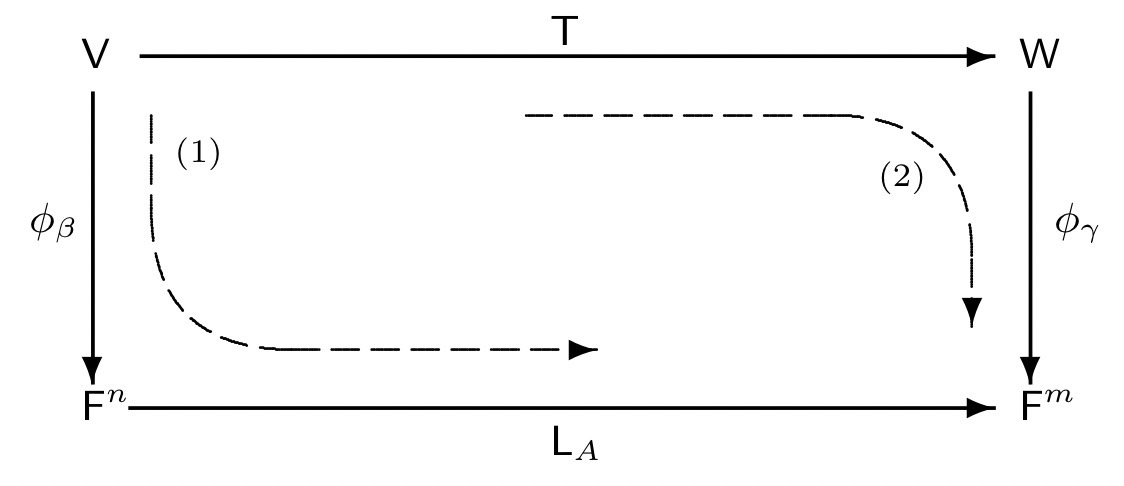
\includegraphics[scale = 0.25]{./figure/105.jpg}
\end{center}



Let $V$ and $W$ be vector spaces of dimension $n$ and $m$, respectively, and let $T: V \rightarrow W$ be a linear transformation. Define $A = [T]^{\gamma}_{\beta}$, where $\beta$ and $\gamma$ are arbitrary ordered bases of $V$ and $W$, respectively. We are now able to use $\phi_{\beta}$ and $\phi \gamma$ to study the relationship between the linear transformations $T$ and $L_A : \mathrm{F}^n \rightarrow \mathrm{F}^m$.
Let us first consider figure above. Notice that there are two composites of linear transformations that map $V$ into $\mathrm{F}^m$:

\begin{enumerate}
	\item Map $V$ into $\mathrm{F}^n$ with $\phi_{\beta}$ and follow this transformation with $L_A$; this yields the composite $L_A\phi_{\beta}$.
	\item Map $V$ into $W$ with $T$ and follow it by $\phi_{\gamma}$ to obtain the composite $\phi_{\gamma}T$.
\end{enumerate}

These two composites are depicted by the dashed arrows in the diagram.
By a simple reformulation of Theorem 2.14 (p. 91), we may conclude that

$$L_A\phi_{\beta} = \phi_{\gamma}T$$


that is, the diagram "commutes." Heuristically, this relationship indicates that after $V$ and $W$ are identified with $\mathrm{F}^n$ and $\mathrm{F}^m$ via $\phi_{\beta}$ and $\phi_{\gamma}$, respectively, we may "identify" $T$ with $L_A$. This diagram allows us to transfer operations on abstract vector spaces to ones on $\mathrm{F}^n$ and $\mathrm{F}^m$.

\begin{thm}% ex 2.4 20
	Let $T:V \rightarrow W$ be a linear transformation from an $n$-dimensional vector space $V$ to an $m$-dimensional vector space $W$. Let $\beta$ and $\gamma$ be ordered bases for $V$ and $W$, respectively. Prove that rank$(T) = $ rank$(L_A)$ and that nullity$(T) = $ nullity($L_A$), where $A = [T]^{\gamma}_{\beta}$.
\end{thm}

\redd{not yet}
